\section{Graphs of Functions}

\begin{definition}[The Fundamental Graphing Principle for Functions]
    The graph of a function $f$ is the set of points which satisfy the equation $y=f(x)$. That is, the point $(x,y)$ is on the graph if and only if $y = f(x)$
\end{definition}

\begin{definition}[Zeros of a function]
    The \textbf{Zeros} of a function $f$ are the solutions to the equation $f(x) = 0$. In other words, $x$ is a zero of $f$ if and only if $(x,0)$ is an $x$-intercept of the graph of $y=f(x)$
\end{definition}

\begin{definition} [Testing the Graph of a Function for Symmetry]
    The graph of a function $f$ is symmetric
    \begin{itemize}
        \item about the $y$-axis if and only if $f(-x)=f(x)$ for all $x$ in the domain of $f$
        \item about the origin if and only if $f(-x) = -f(x)$ for all $x$ in the domain of $f$
    \end{itemize}
\end{definition}

\subsection{General Function Behavior}

\begin{definition}[Increasing, Decreasing and Constant Functions]
    Suppose $f$ is a function defined on an interval $I$. We say $f$ is:
    \begin{itemize}
        \item \textbf{increasing} on $I$ if and only if $f(a) < f(b)$ for all real numbers $a, b \in I (a<b)$
        \item \textbf{decreasing} on $I$ if and only if $f(a) > f(b)$ for all real numbers $a, b \in I (a<b)$
        \item \textbf{constant} on $I$ if and only if $f(a) = f(b)$ for all real numbers $a, b \in I$
    \end{itemize}
\end{definition}

\begin{definition}[Maximums and Minimums of a Function]
    Suppose that $f$ is a function with $f(a) = b$
    \begin{itemize}
        \item We say $f$ has a \textbf{local maximum} at the point $(a,b)$ if and only if there is an open interval $I$ containing $a$ for which $f(a) \geq f(x)$ for all $x \in I$. The value $f(a) = b$ is called 'a local maximum value of f' in this case.
        \item We say $f$ has a \textbf{local minimum} at the point $(a,b)$ if and only if there is an open interval $I$ containing $a$ for which $f(a) \leq f(x)$ for all $x \in I$. The value $f(a) = b$ is called 'a local minimum value of f' in this case.
        \item The value $b$ is called the \textbf{maximum} of $f$ if $b \geq f(x)$ for all $x$ in the domain of $f$
        \item The value $b$ is called the \textbf{minimum} of $f$ if $b \leq f(x)$ for all $x$ in the domain of $f$
    \end{itemize}
\end{definition}

\subsection{Problems}
\begin{enumerate}
    \item[1.] Domain $(-\infty, \infty)$, intercepts: $(2,0)$, Not symmetric
          \leavevmode
          \begin{center}
              
\includegraphics[width=0.5\textwidth]{figures/01_Relations_and_Functions/06_Graphs_of_Functions/exercise_1.pdf}
          \end{center}
    \item[4.] Domain $(-\infty, \infty)$, intercepts: $(-2,0), (2,0)$, Symmetric about the $y$-axis
          \leavevmode
          \begin{center}
              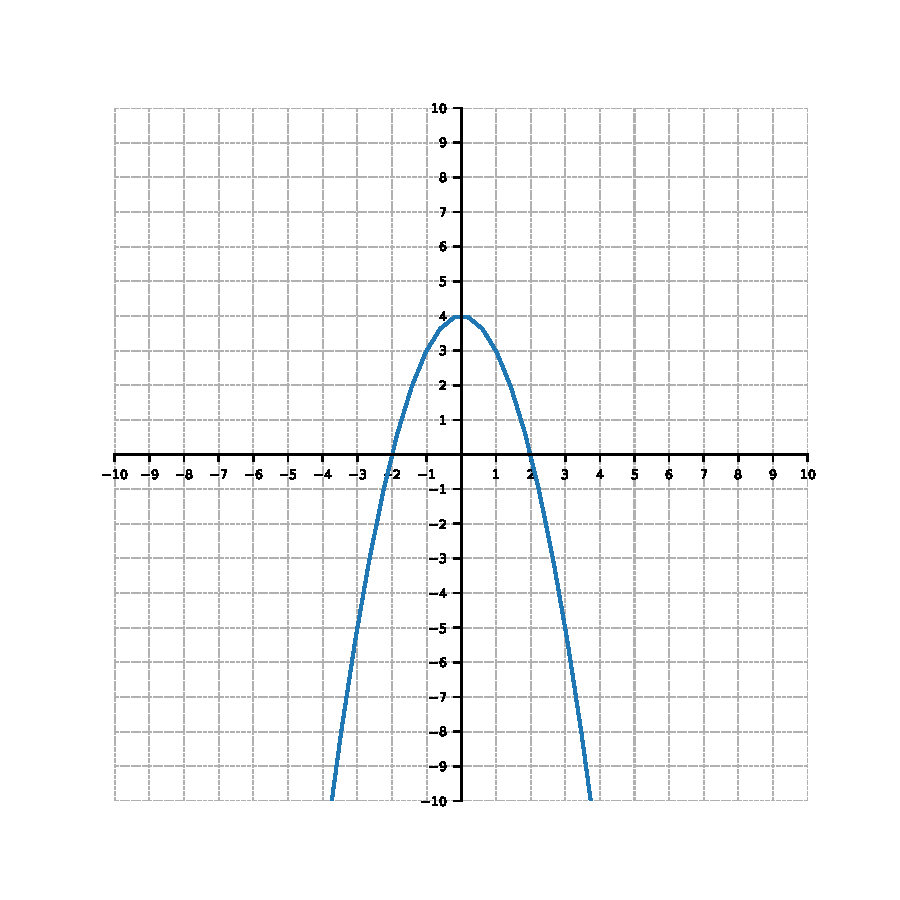
\includegraphics[width=0.5\textwidth]{figures/01_Relations_and_Functions/06_Graphs_of_Functions/exercise_4.pdf}
          \end{center}
    \item[13.] \leavevmode
          \begin{center}
              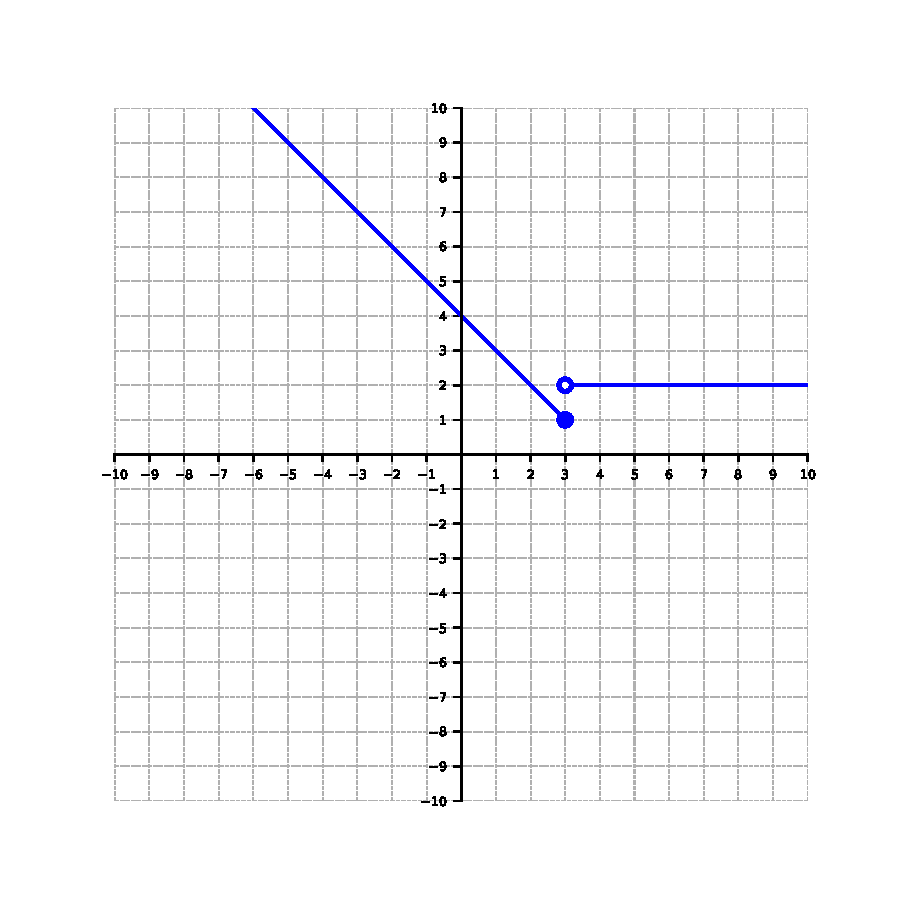
\includegraphics[width=0.5\textwidth]{figures/01_Relations_and_Functions/06_Graphs_of_Functions/exercise_13.pdf}
          \end{center}
    \item[21.] Neither even nor odd.
          \[
              f(x) = 7x \neq -7x = f(-x); f(x) = 7x \neq -7x = -f(x)
          \]
    \item[28.] Function is even
          \[
              f(x) = 4 - x^2 = f(-x); f(x) = 4-x^2 \neq = x^2 - 4 = -f(x)
          \]
\end{enumerate}